\chapter{Complete plots of data}
\section{Raw parasite counts}
\begin{sidewaysfigure}
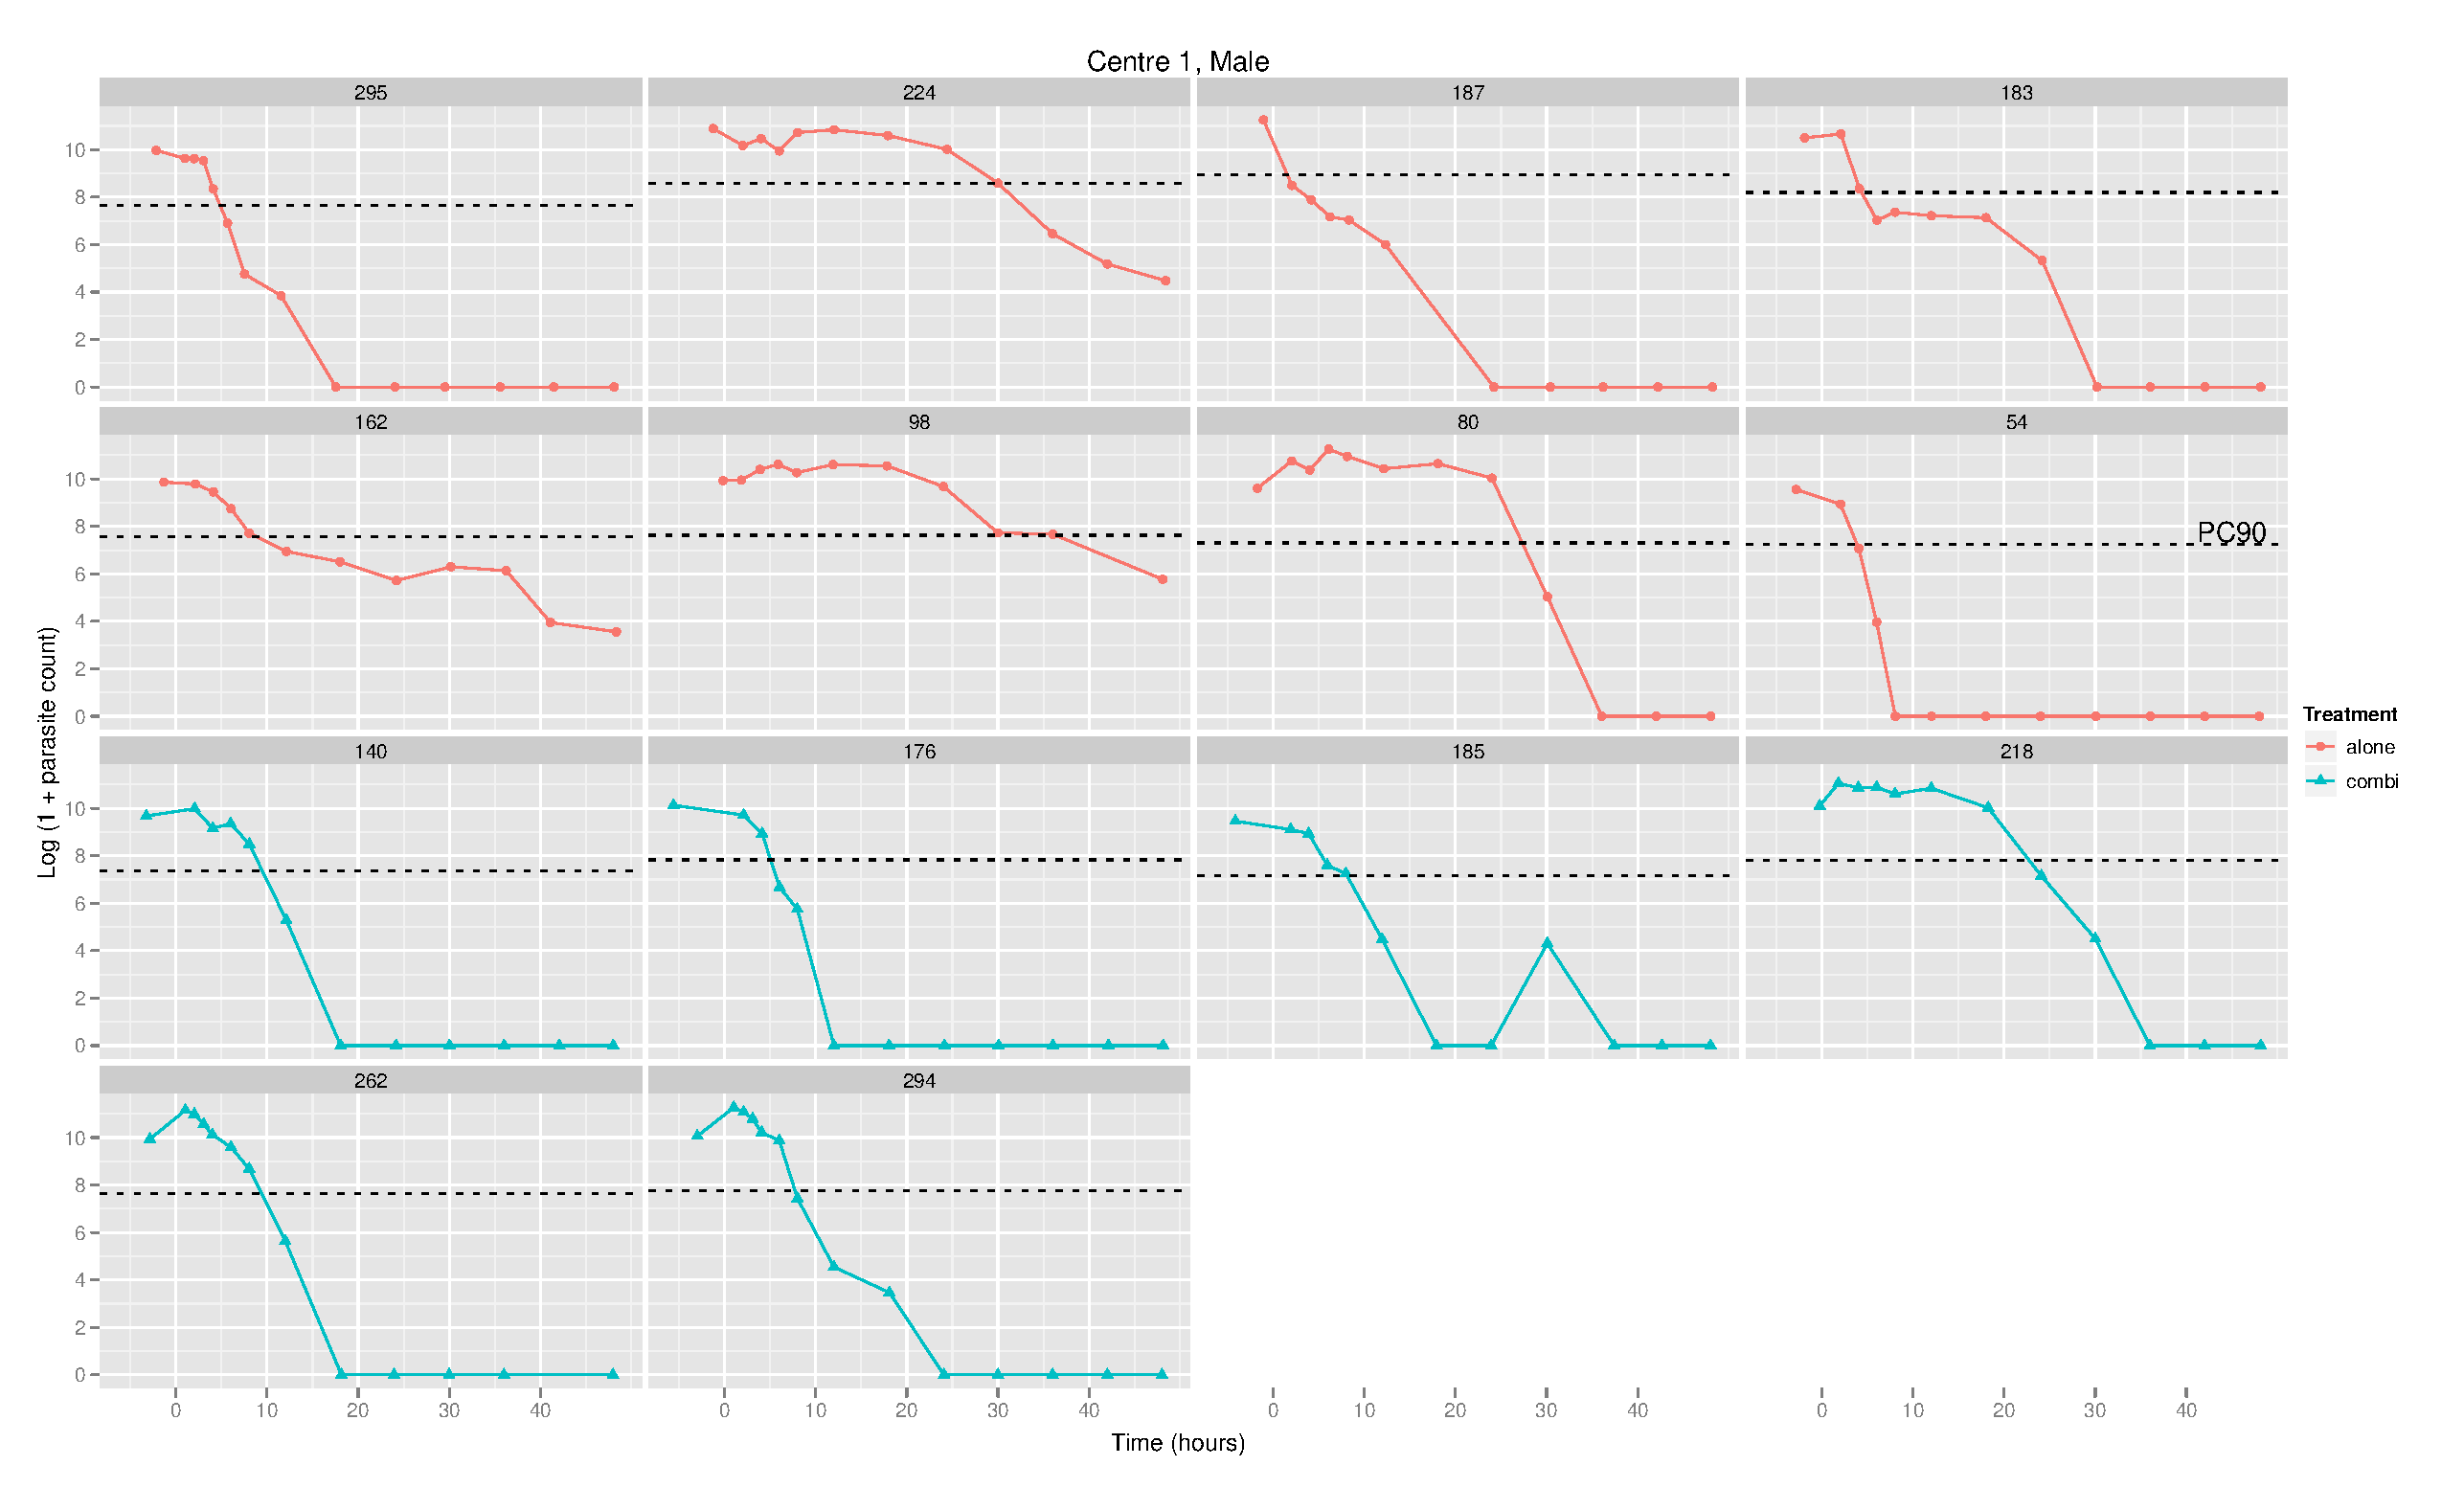
\includegraphics[height=150mm]{Araw1M.eps}
\end{sidewaysfigure}
\begin{sidewaysfigure}
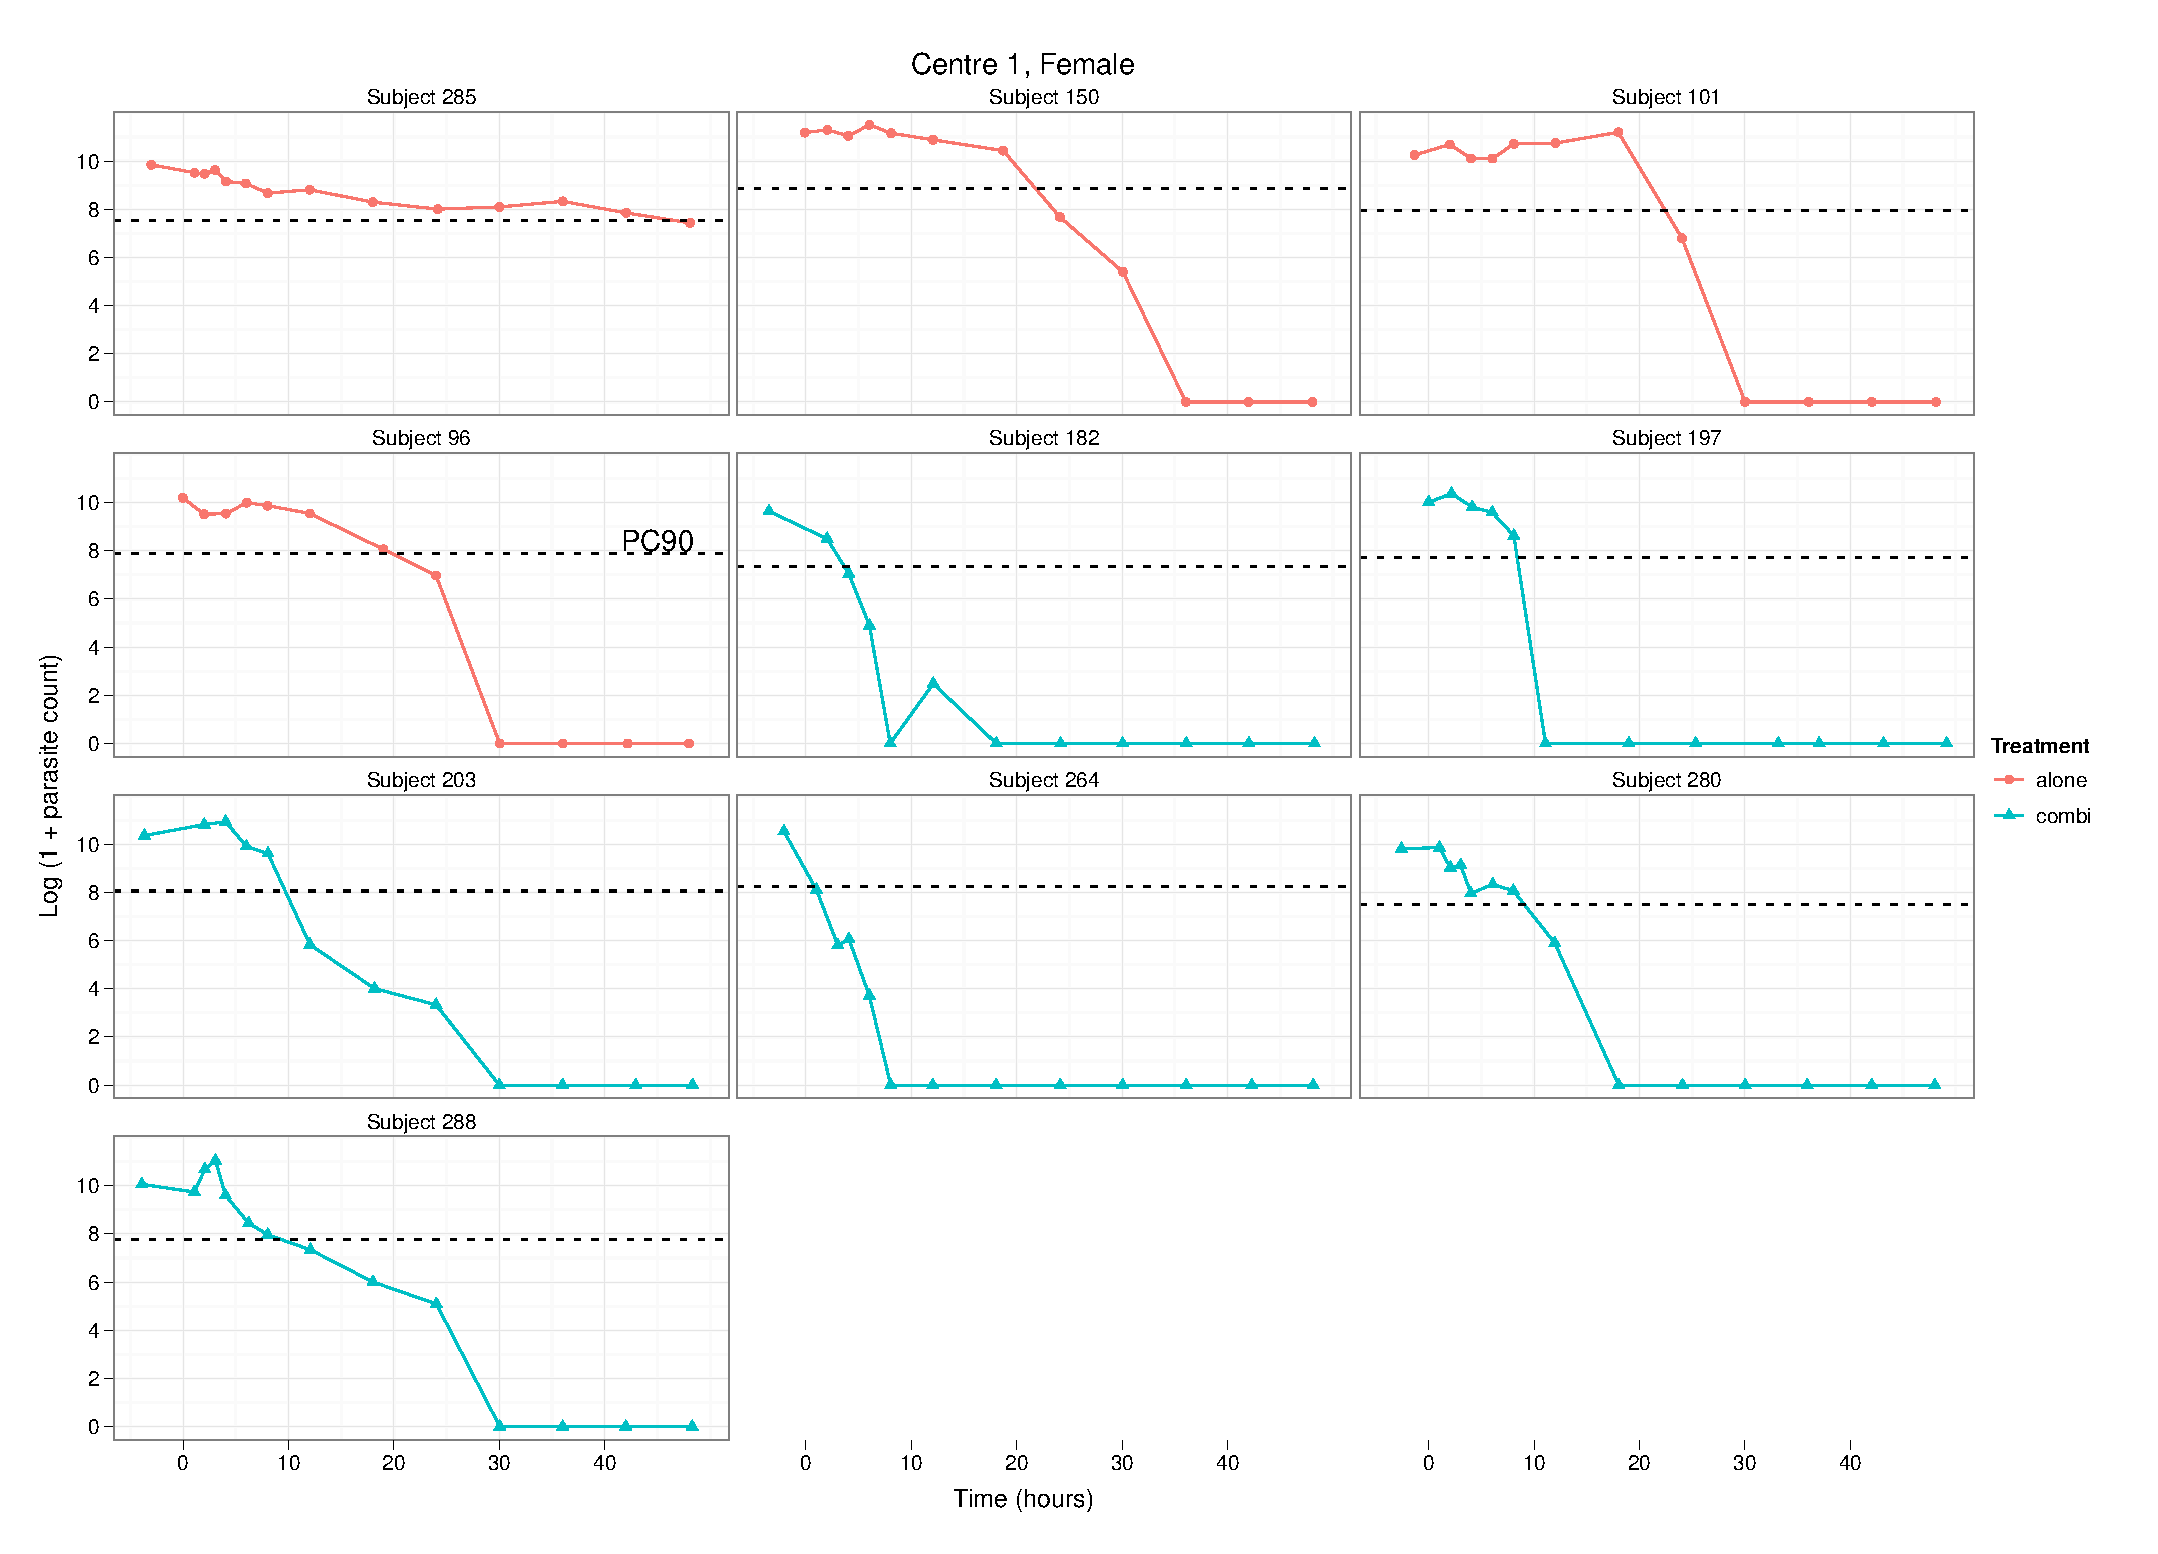
\includegraphics[height=150mm]{Araw1F.eps}
\end{sidewaysfigure}
\begin{sidewaysfigure}
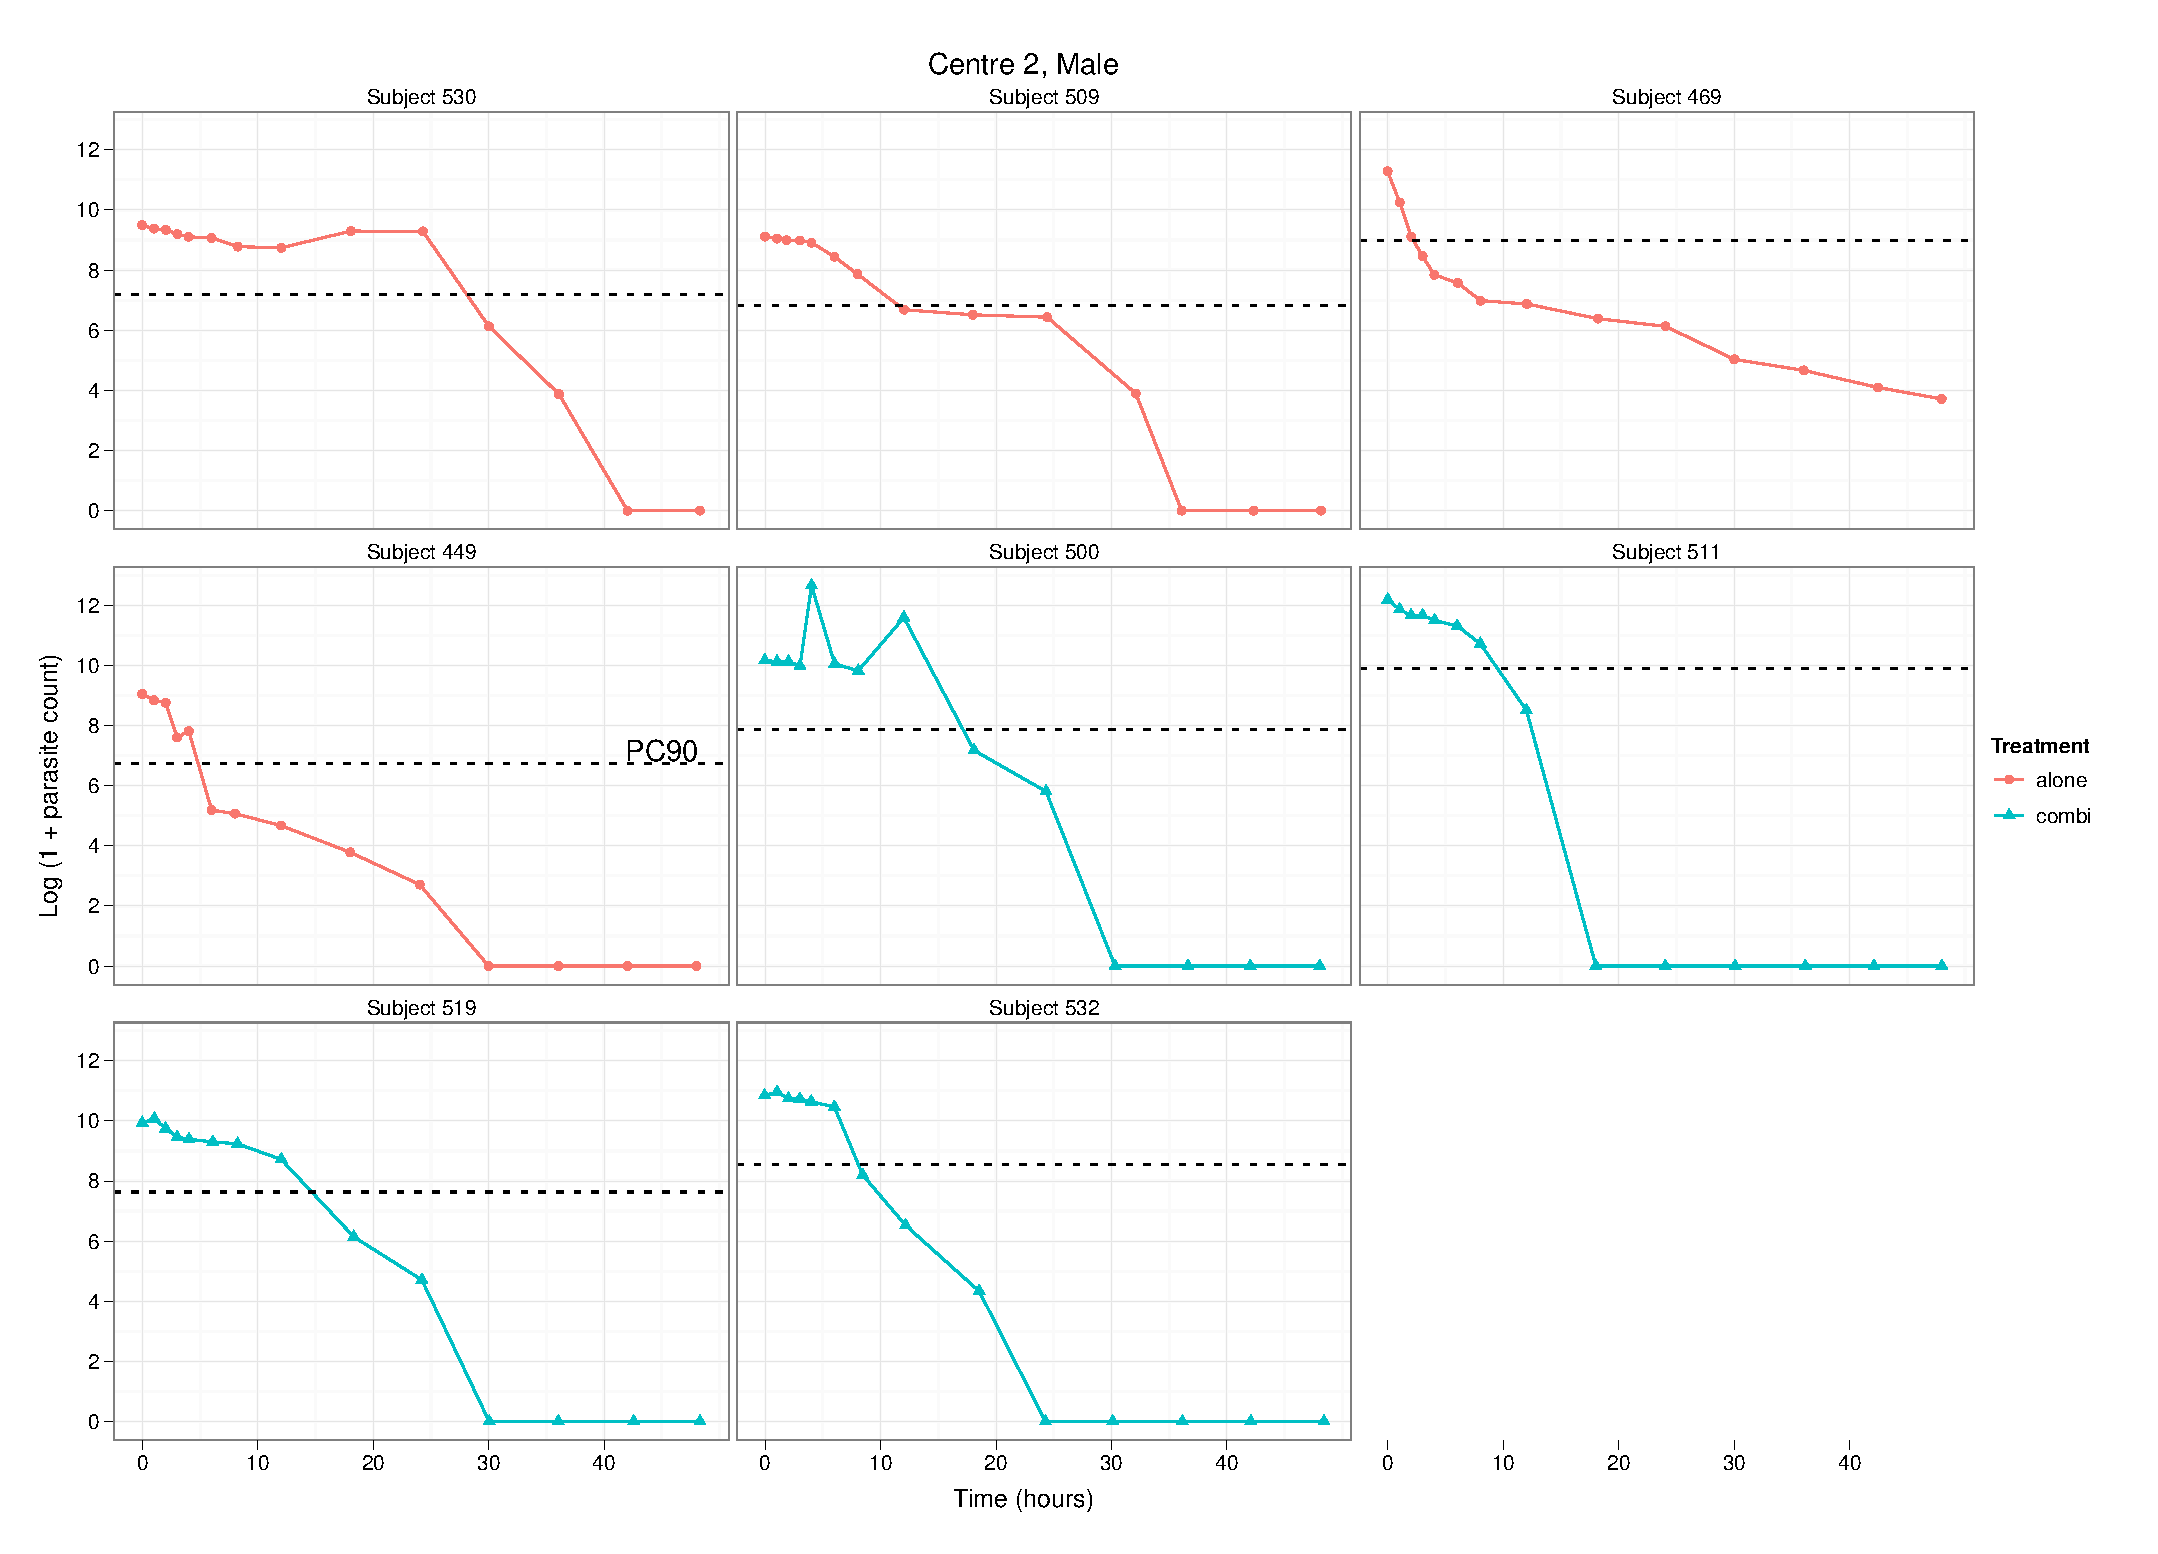
\includegraphics[height=150mm]{Araw2M.eps}
\end{sidewaysfigure}
\begin{sidewaysfigure}
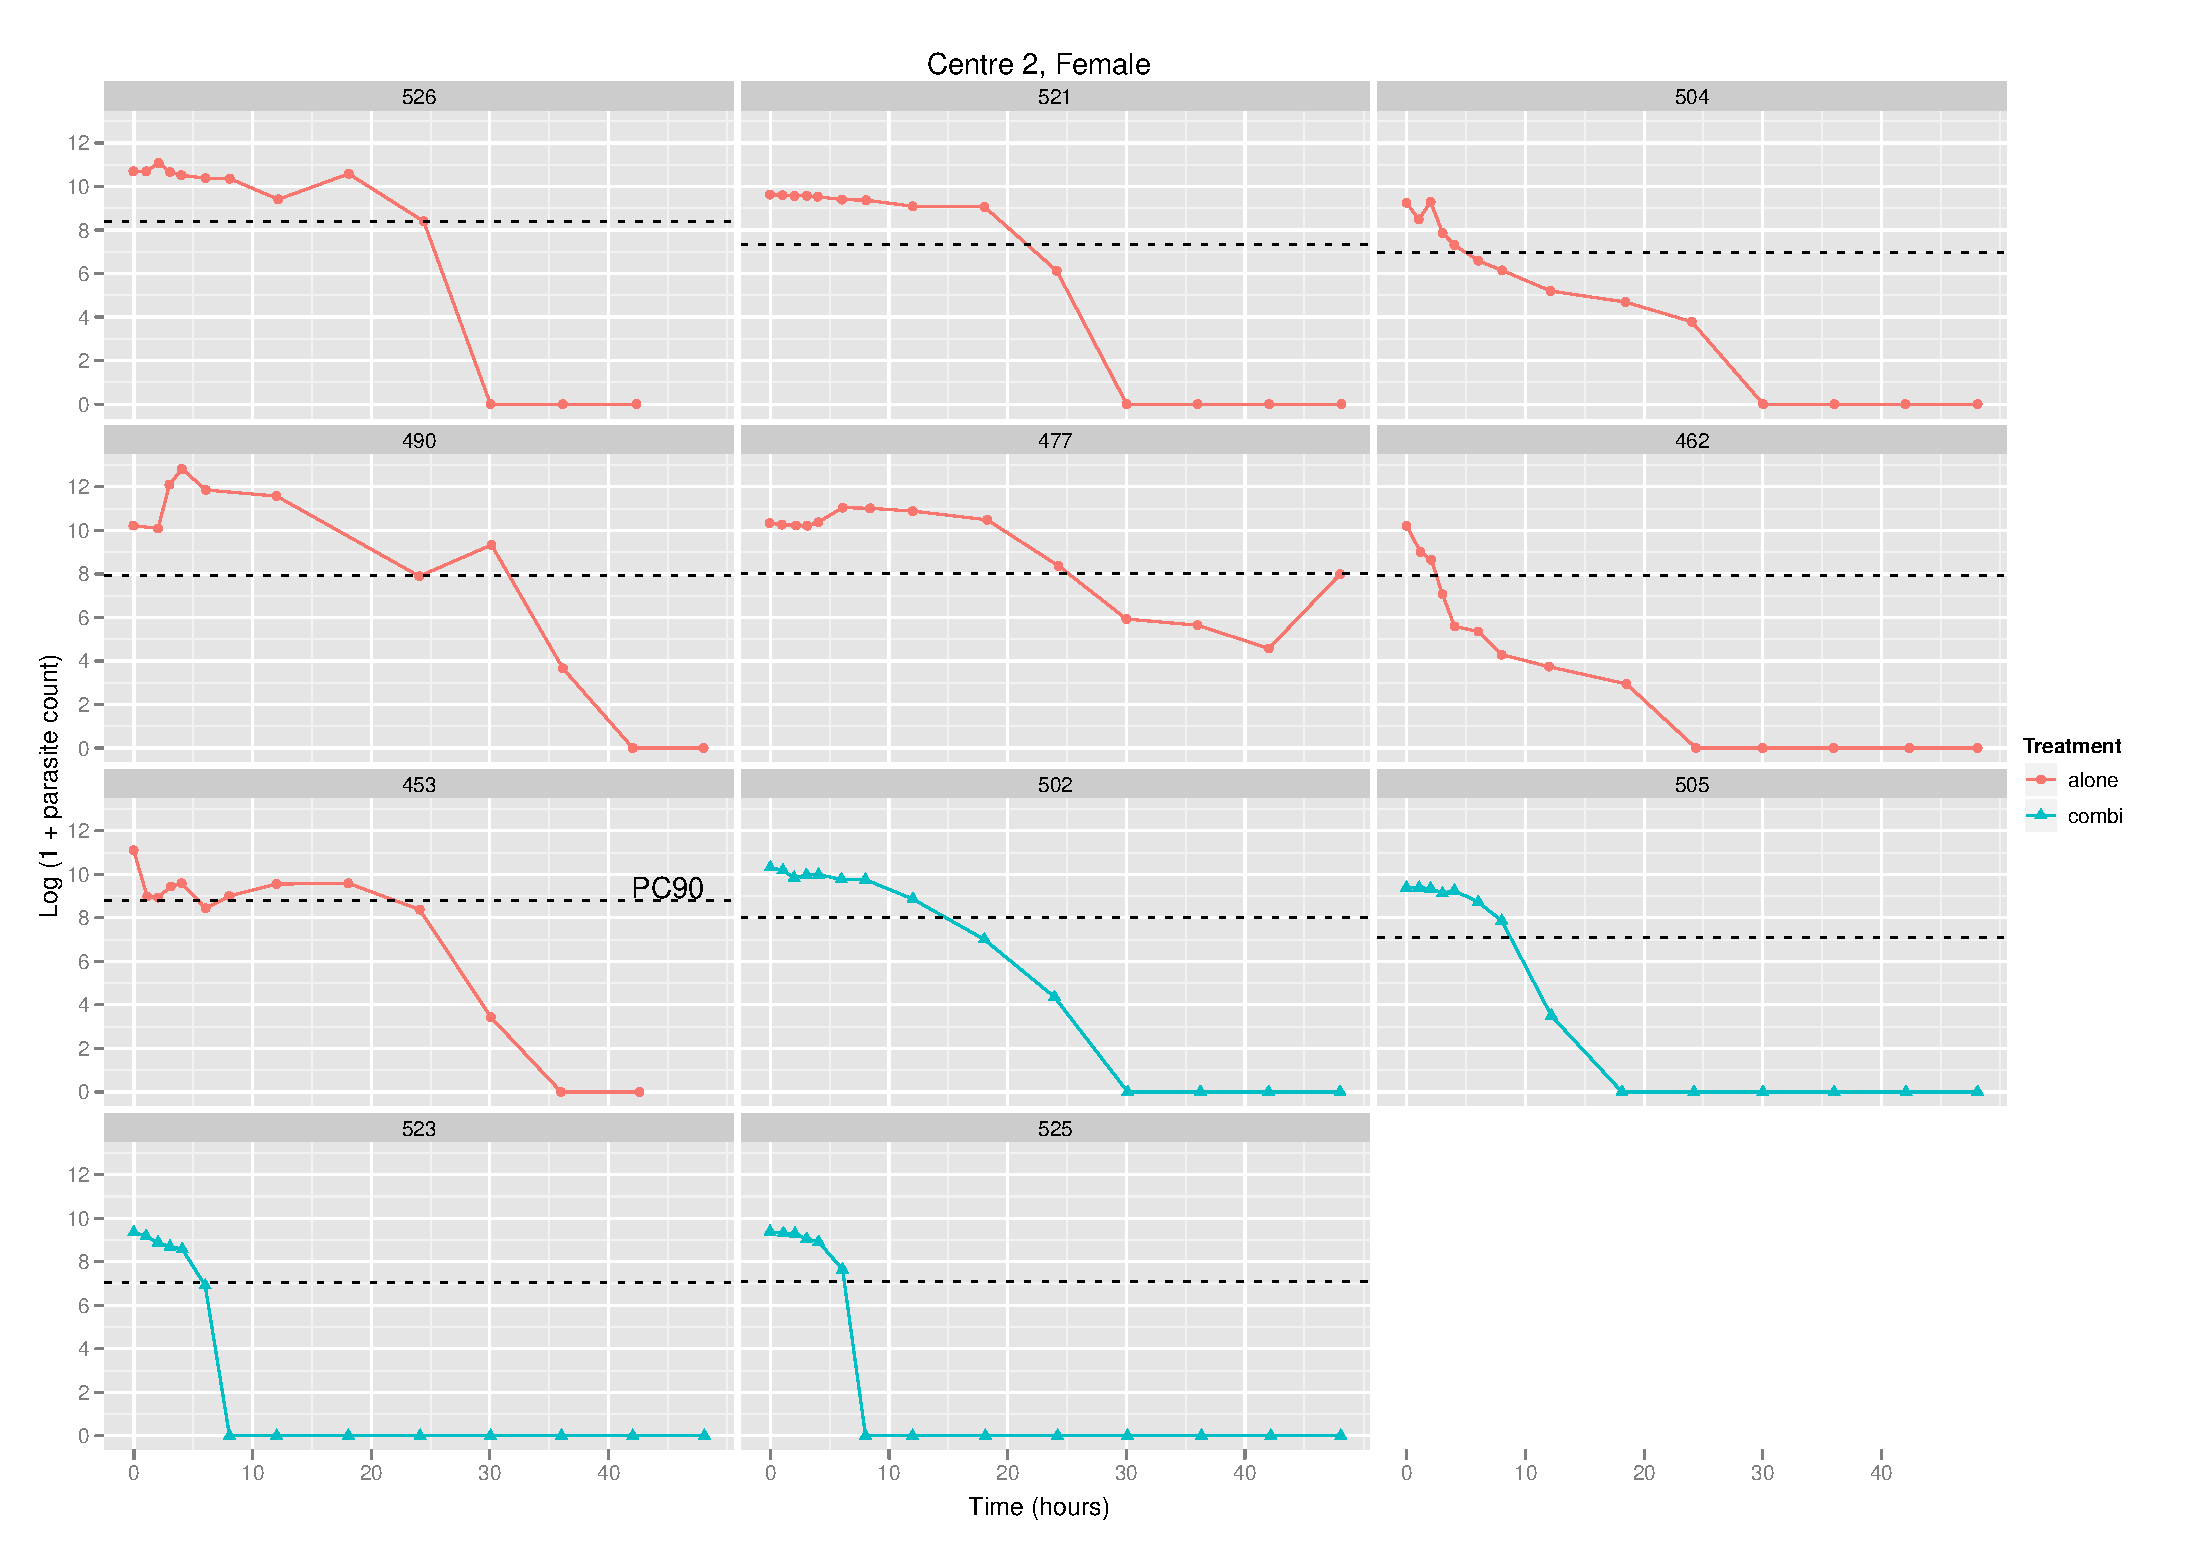
\includegraphics[height=150mm]{Araw2F.eps}
\end{sidewaysfigure}

\clearpage
\section{Model fits}
\begin{sidewaysfigure}
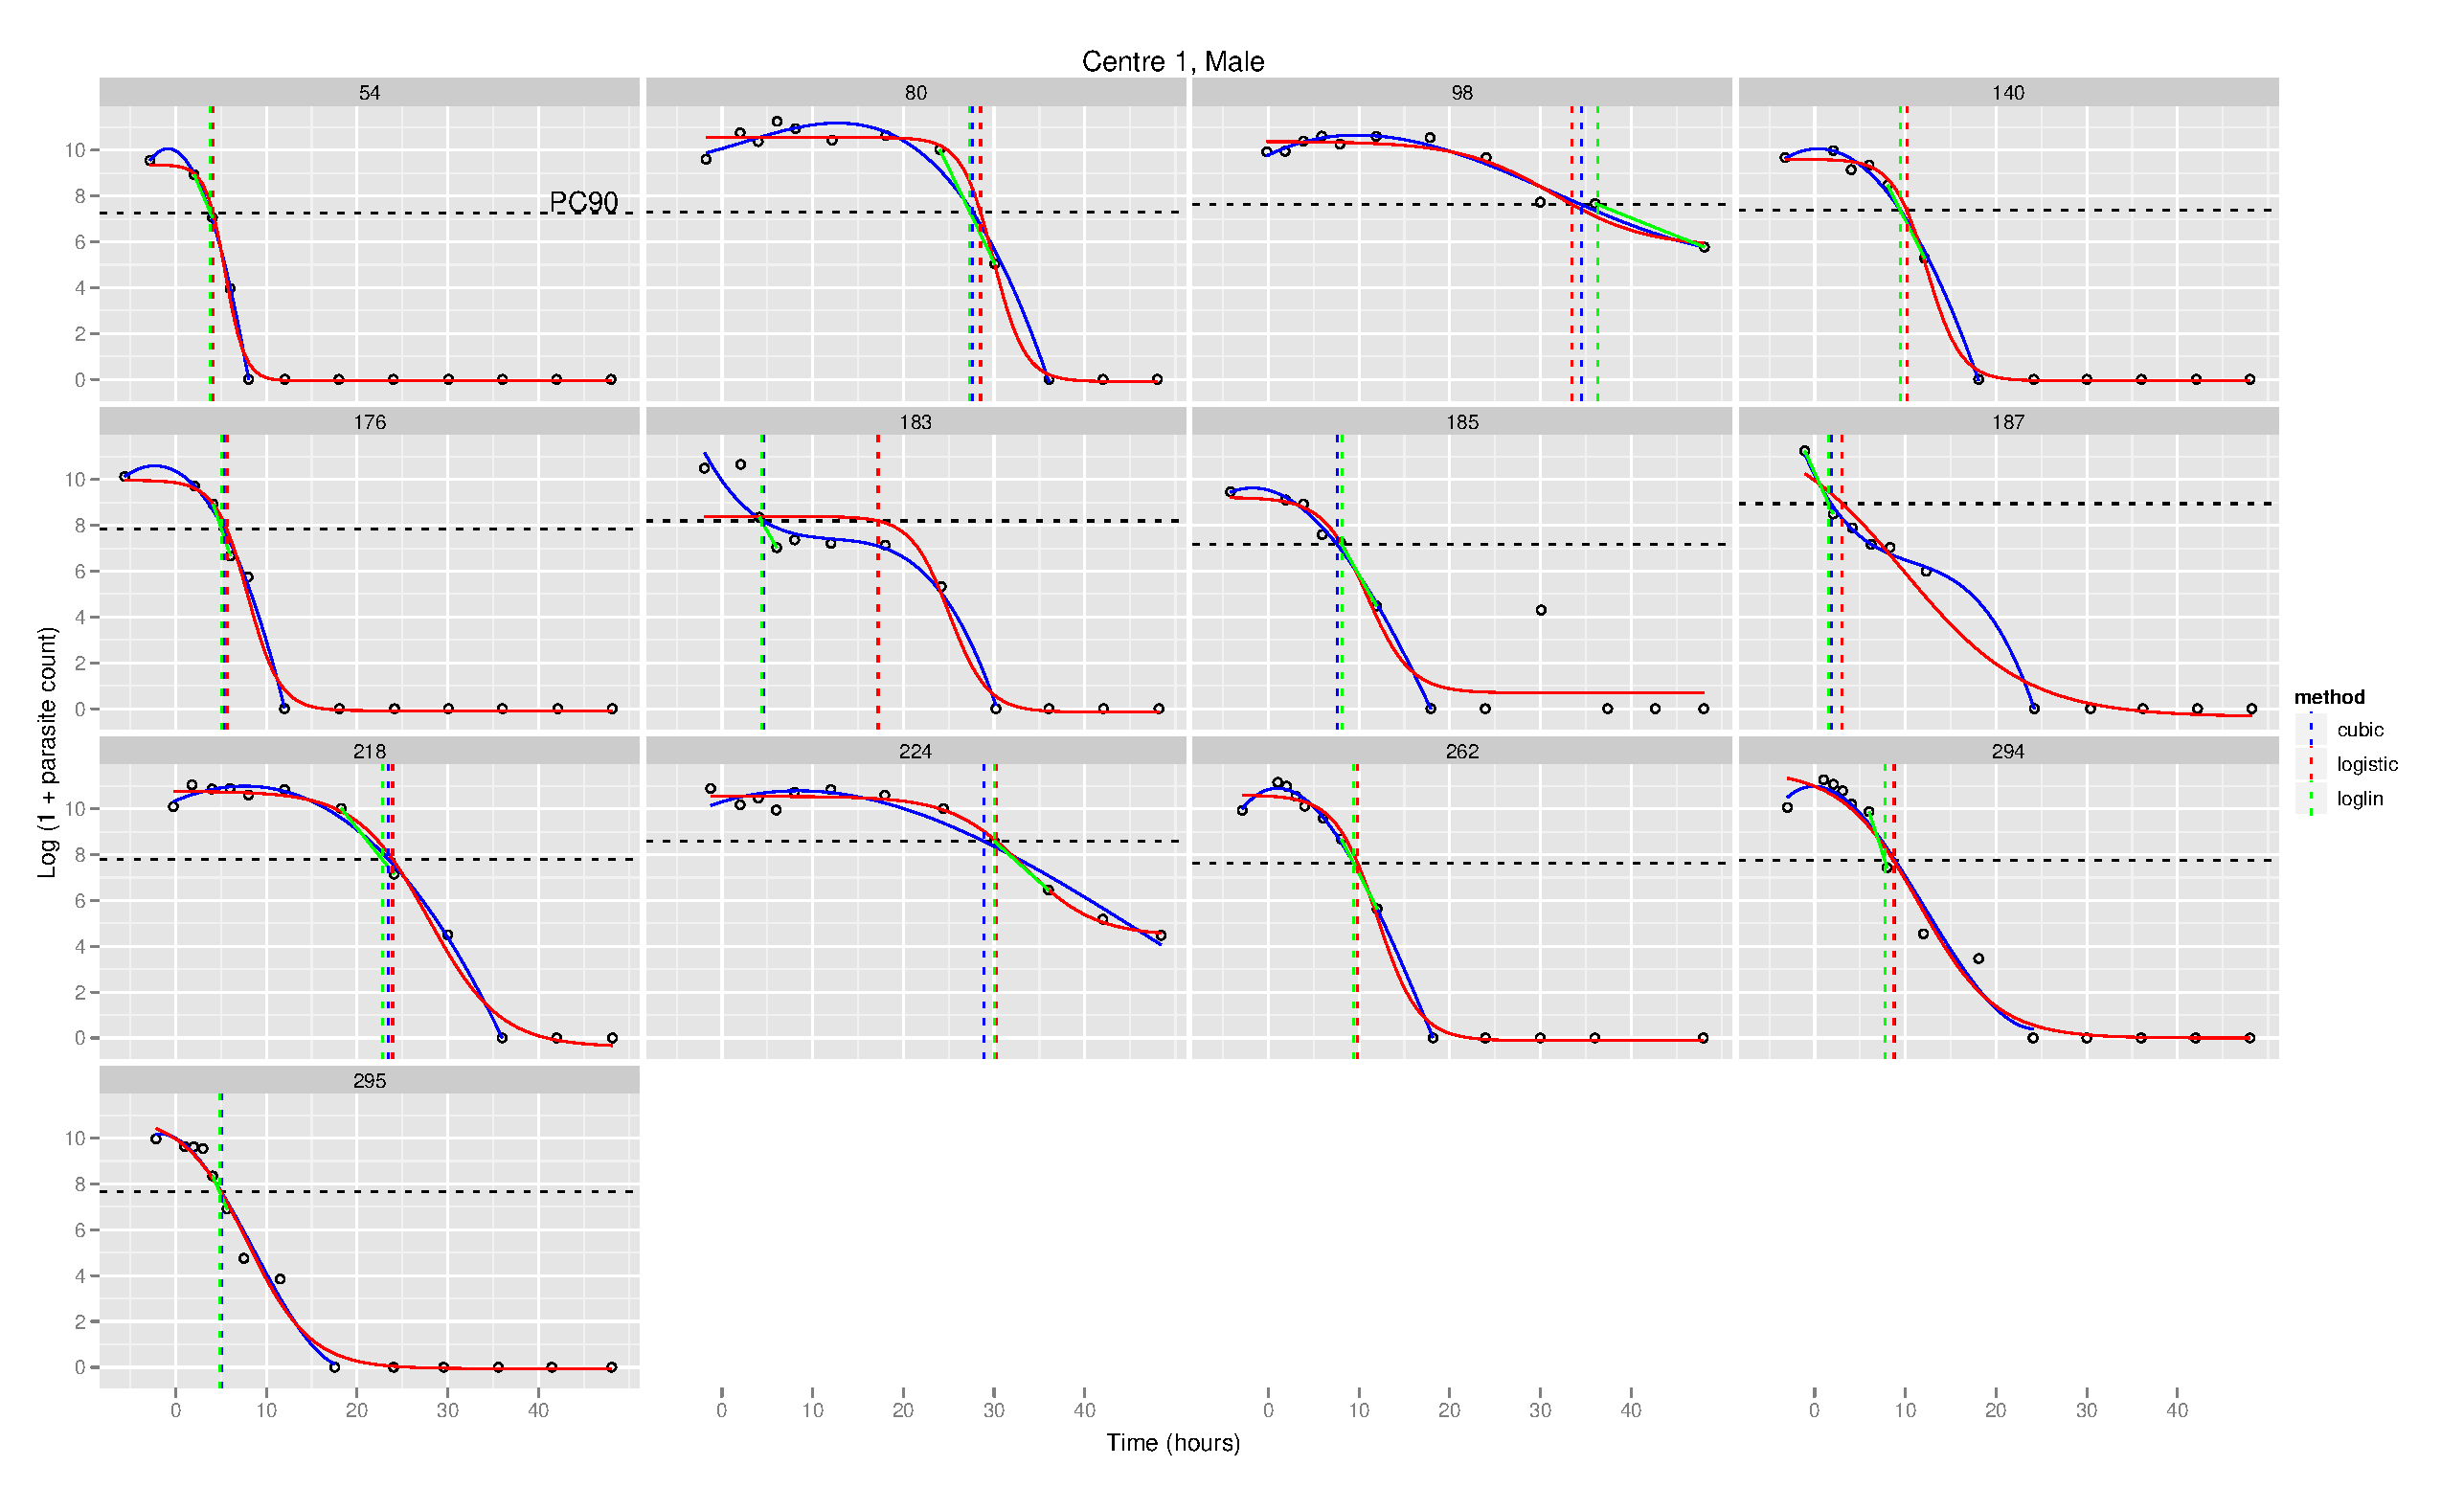
\includegraphics[height=150mm]{Afits1M.eps}
\end{sidewaysfigure}
\begin{sidewaysfigure}
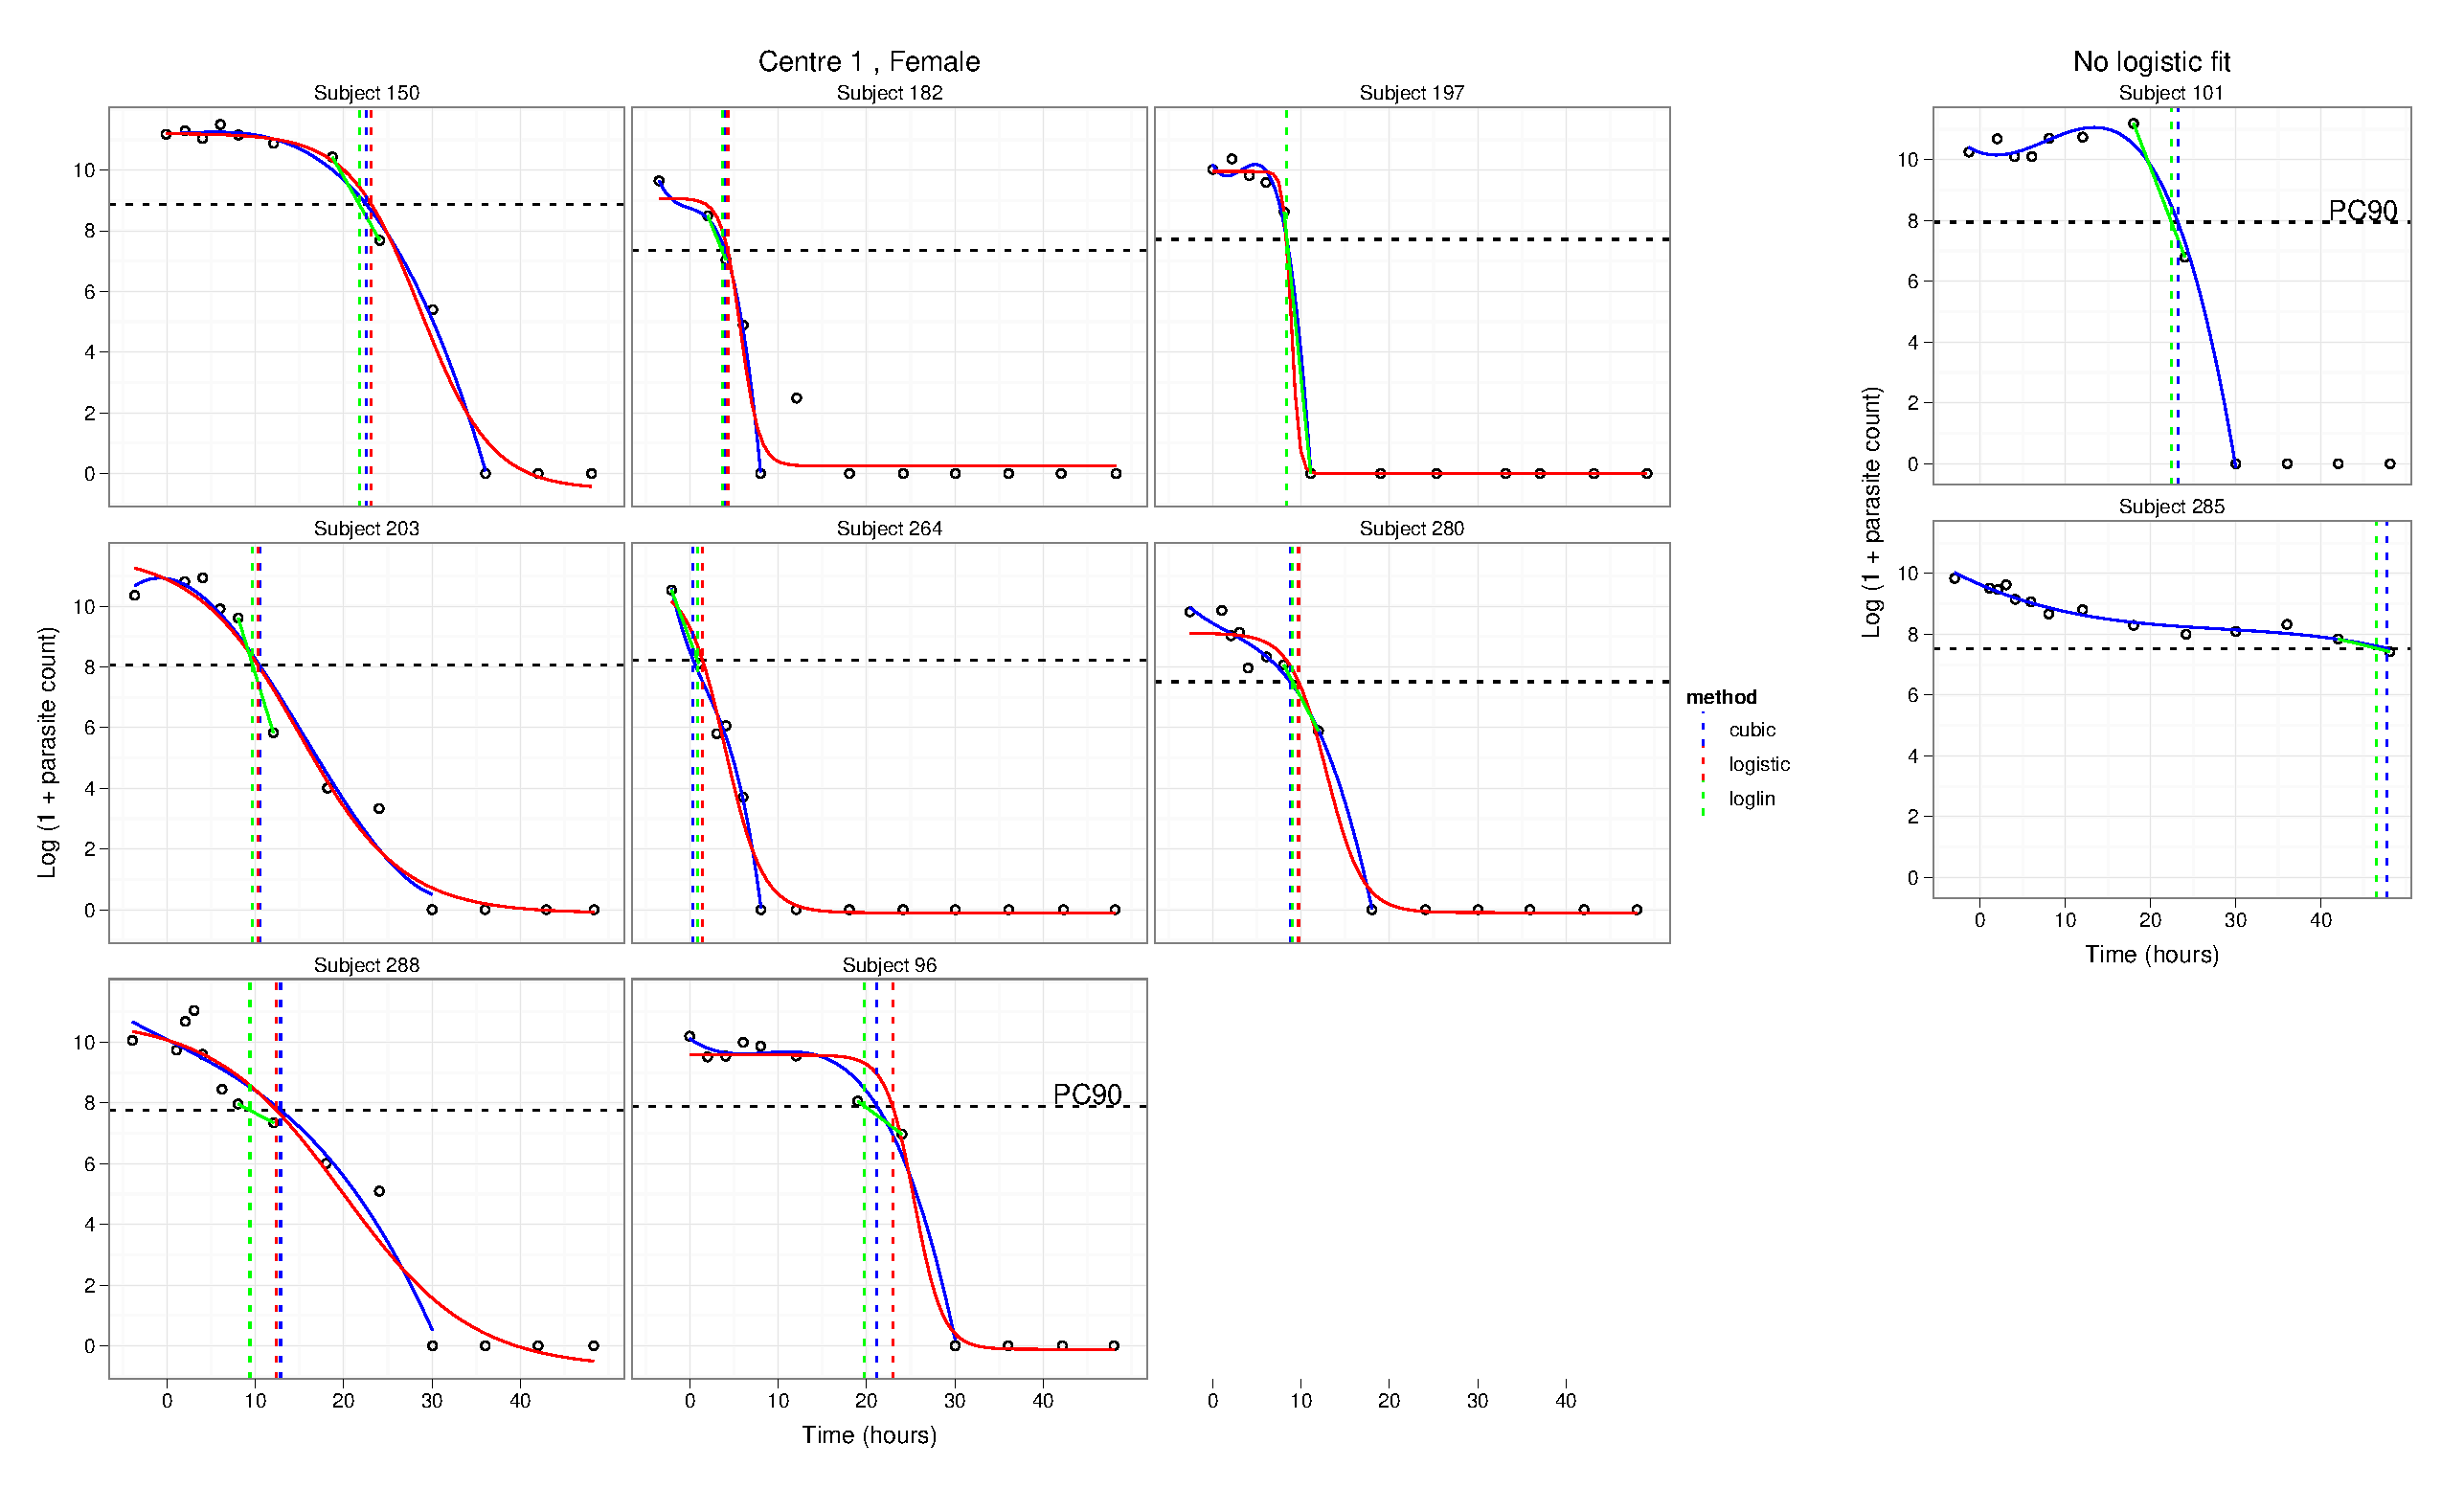
\includegraphics[height=150mm]{Afits1F.eps}
\end{sidewaysfigure}
\begin{sidewaysfigure}
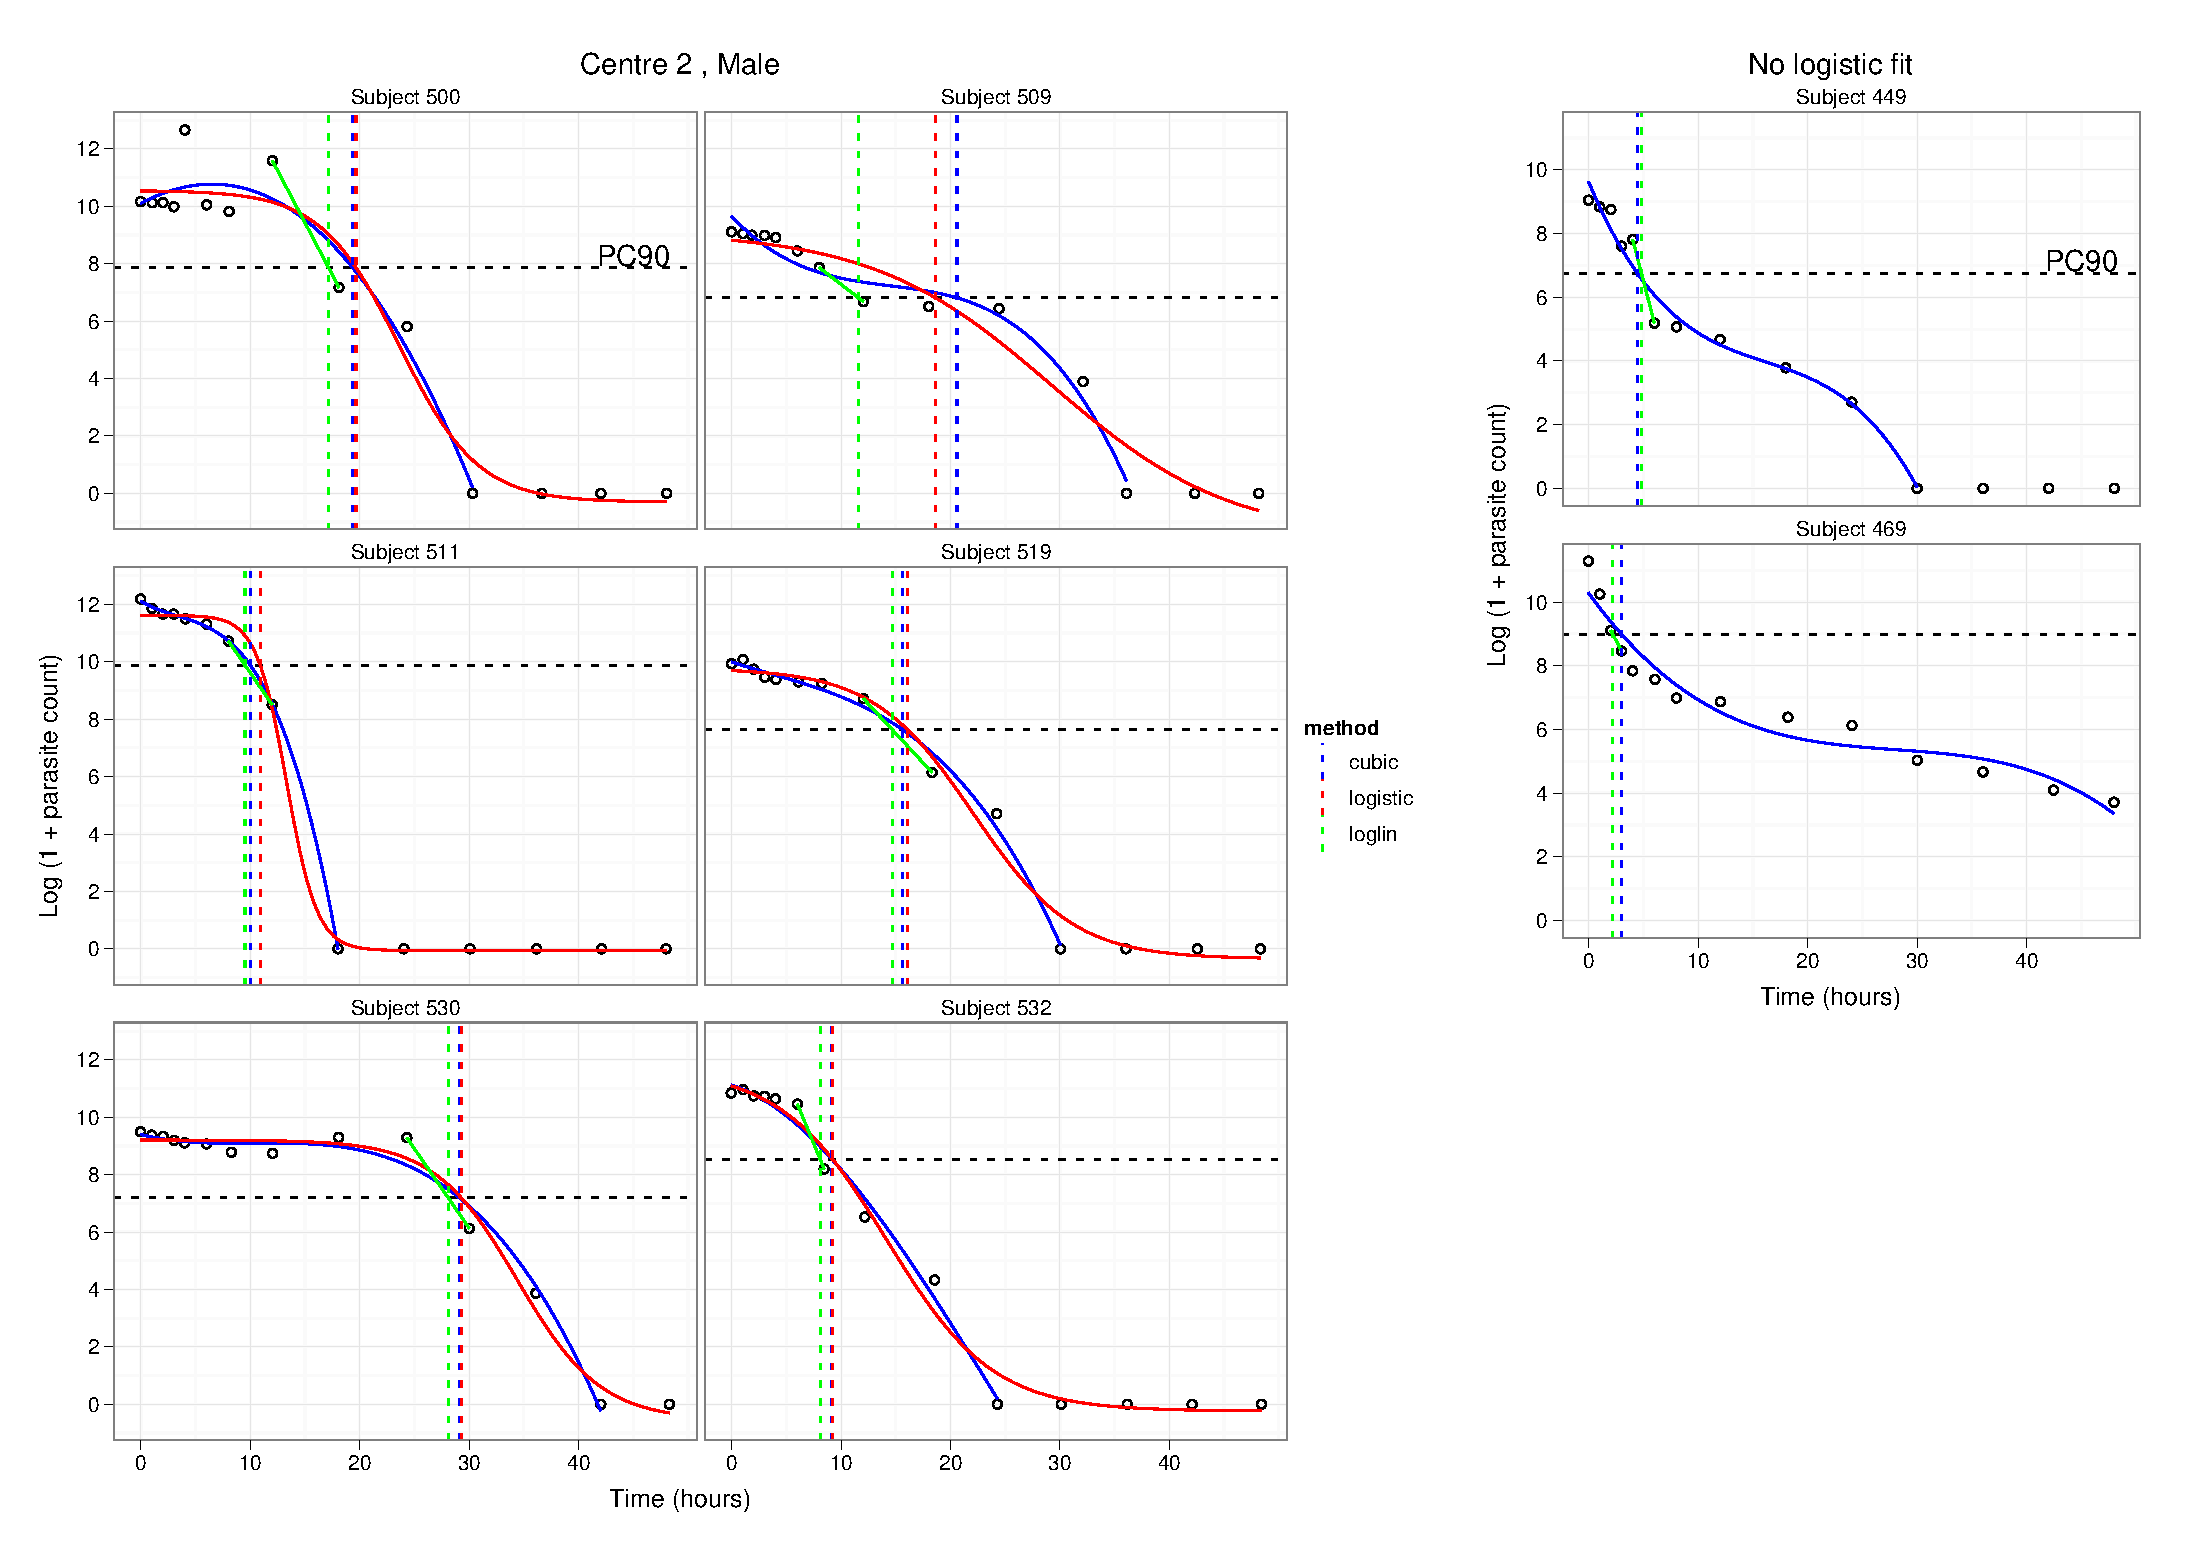
\includegraphics[height=150mm]{Afits2M.eps}
\end{sidewaysfigure}
\begin{sidewaysfigure}
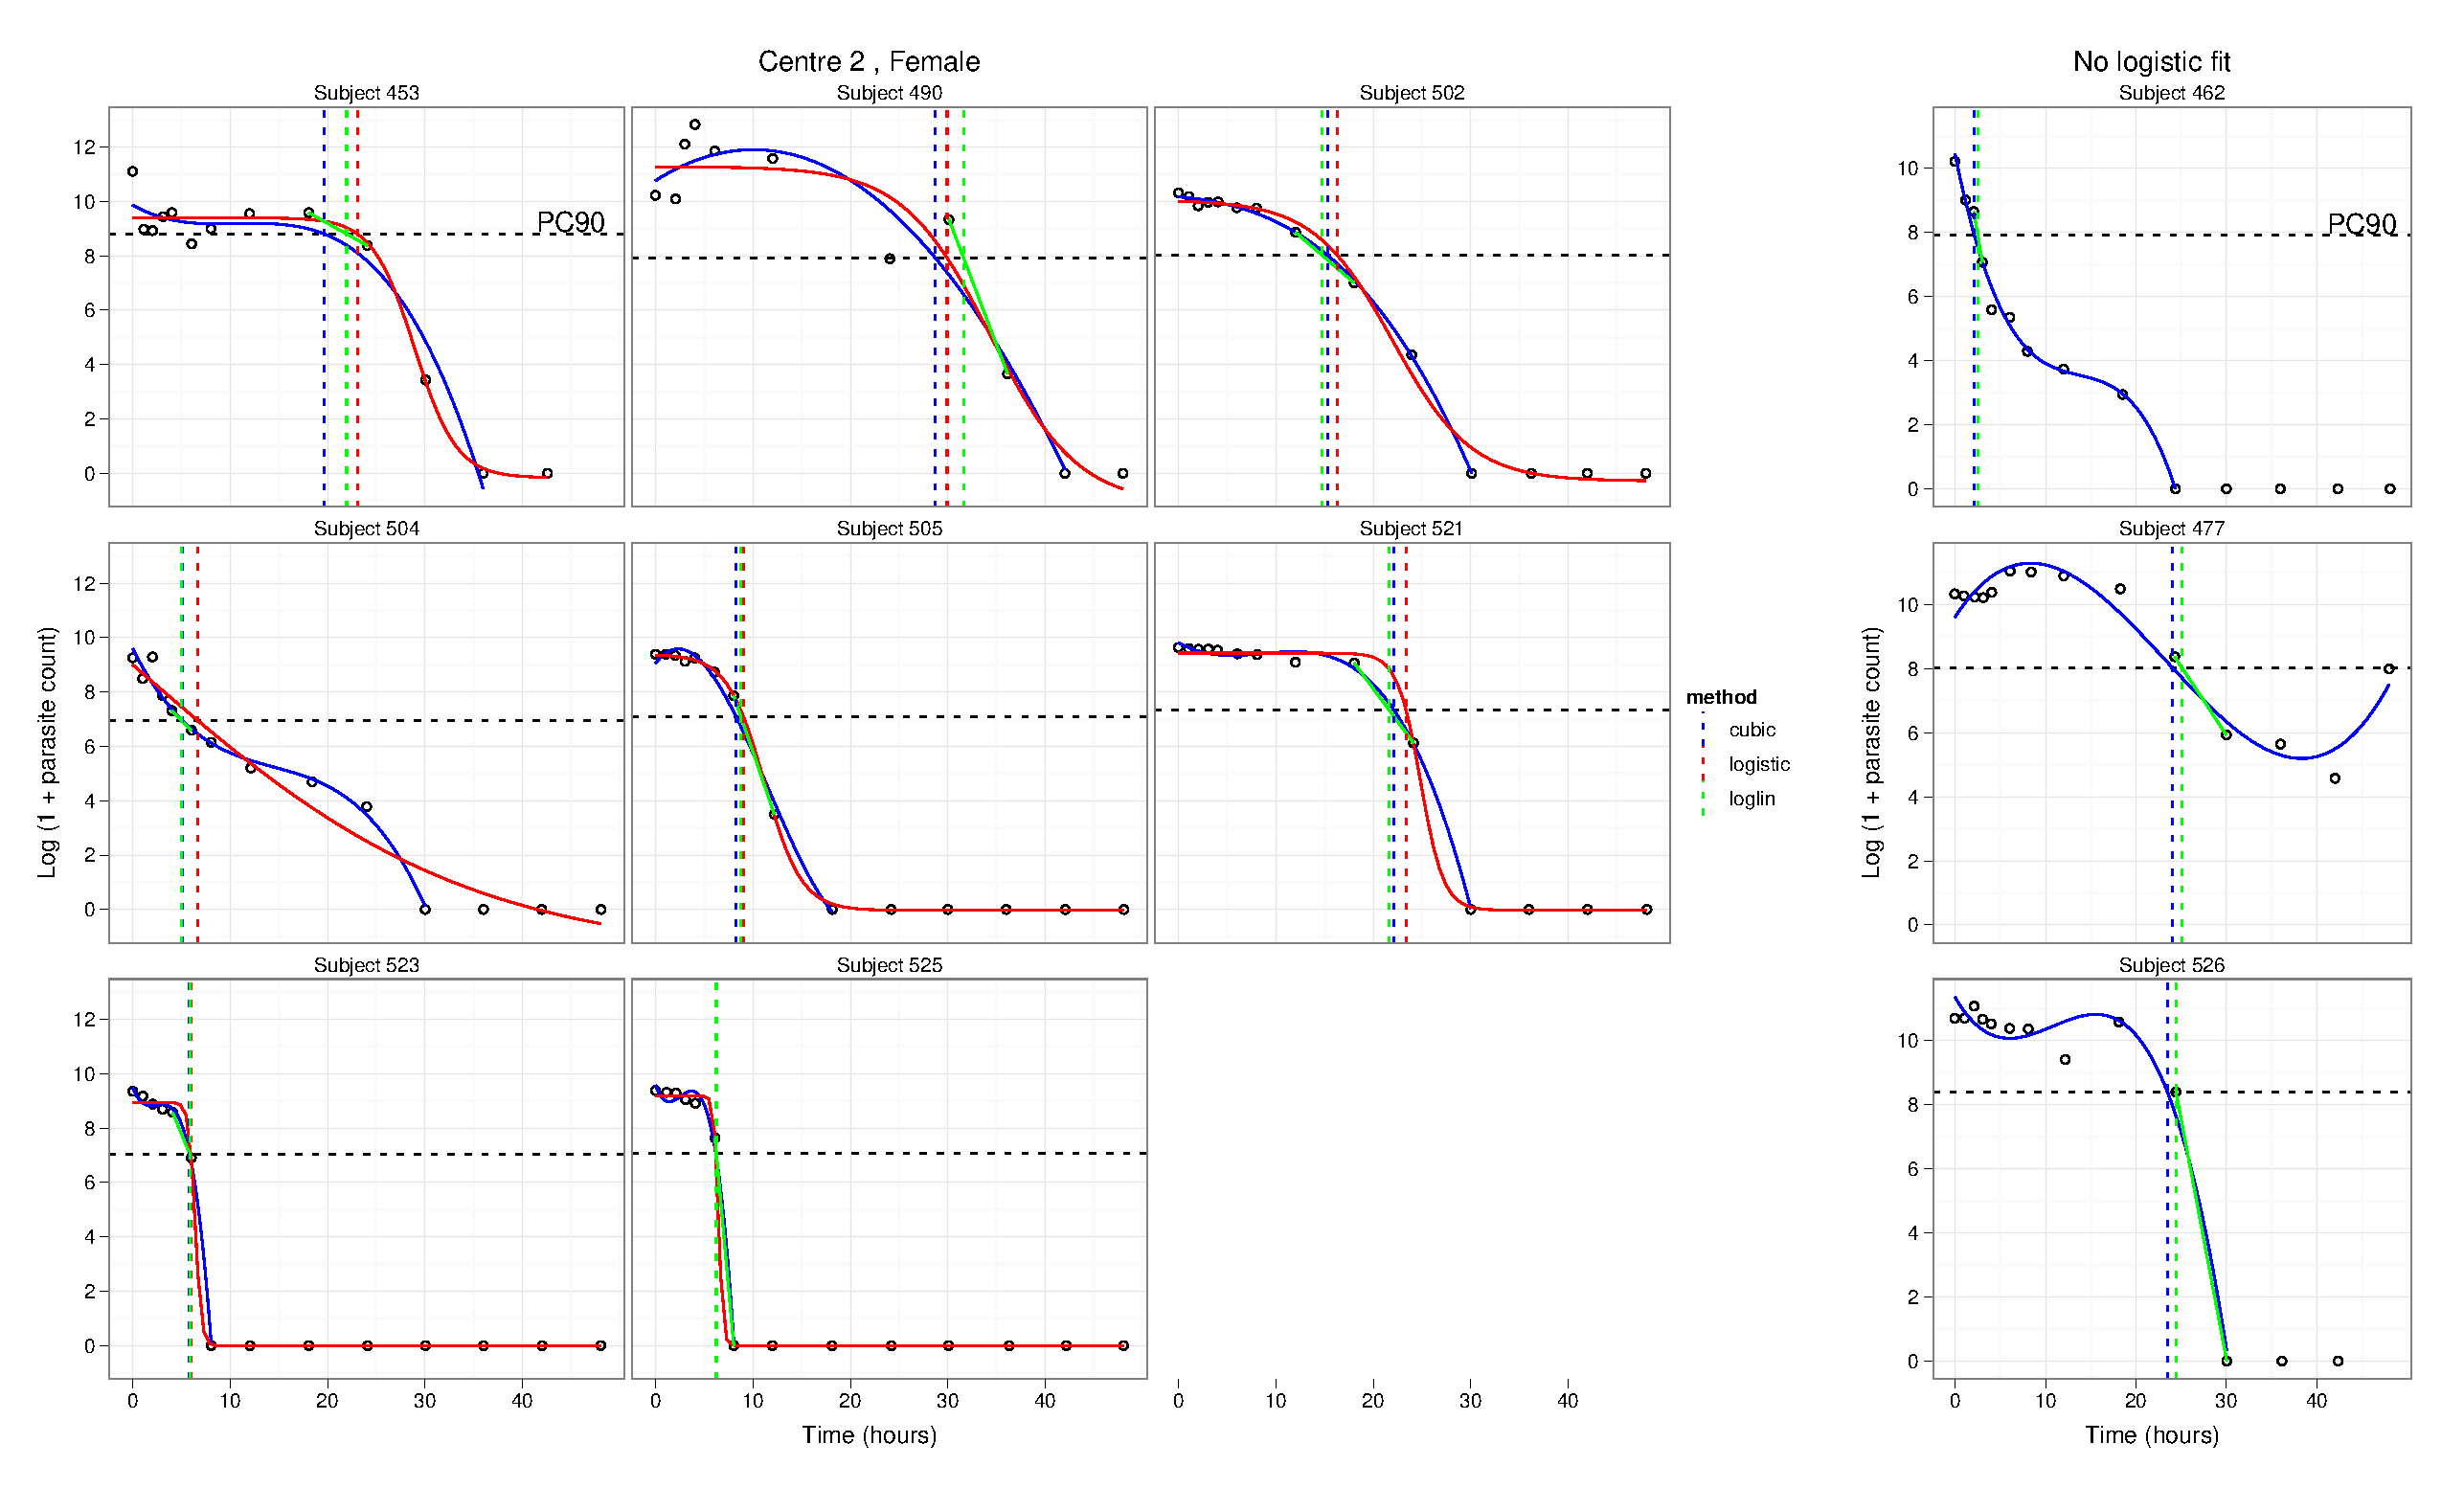
\includegraphics[height=150mm]{Afits2F.eps}
\end{sidewaysfigure}

\chapter{\emph{R} code listings}
\lstset{numberstyle=\small,
frame=single,
framesep=6pt,
tabsize=2,
basicstyle=\small\ttfamily,
%keywordstyle=\bfseries,
%keywordstyle=\color{blue},
%commentstyle=\itshape\color{red},
showstringspaces=false,
columns = fullflexible,
language=R,
breaklines=true,
showstringspaces=false,
lineskip=-1pt}

\section{Functions for PC90 estimation}
\begin{lstlisting}[float=h,caption=Functions to find PC90 by cubic regression,label=R:cubics]
# Create a list of cubic fits to data up to first zero
cubic.fits <- function(data) {
	require(nlme)
	lmList(log(1 + parct) ~ acttm + I(acttm^2) + I(acttm^3) | SUBJID, data=uptofirstzero(data))
}

# Create a new data frame containing data up to first zero count
uptofirstzero <- function(data) {
	new.df <- data.frame()
	for (s in unique(data$SUBJID)) {
		rows <- data[data$SUBJID==s,]
		n <- match(0, rows$parct)
		if (!is.na(n)) {
			rows <- rows[1:n,]
		}
		new.df <- rbind(new.df, rows)
	}
	new.df
}

# Find the PC90 time from a cubic fit
pc90cubic <- function(fit, data) {
	coefs <- coef(fit)
	parct90 <- log(1 + (data$parct[data$plantm=='PRE-DOSE'] * 0.1))
	preds <- predict(fit)
	
	# Find the times at which counts are above and below PC90 
	upper <- which.min(preds > parct90)
	lower <- upper - 1
	interval <- c(data$acttm[lower], data$acttm[upper])

	# Search for PC90 between these times
	soln <- uniroot(function(x) coefs[1] + coefs[2]*x + coefs[3]*x^2 + coefs[4]*x^3 - parct90, interval=interval)
	soln$root
}
\end{lstlisting}

\begin{lstlisting}[float=h,caption=Functions to find PC90 by logistic regression,label=R:logistics]
# Perform logistic fitting after selecting starting parameters
logistic.fit <- function(dat) {
	# Set alpha and lambda to max and min counts
	initA <- max(log(1 + dat$parct))
	initL <- min(log(1 + dat$parct))

	# Set mu to time closest to half max count
	halfway <- (initA + initL)/2
	initU <- dat$acttm[which.min(abs(log(1 + dat$parct) - halfway))]

	# Set beta to -0.5 i.e. 2 in SSfpl formulation
	initB <- 2
	
	tryCatch(fit <- nls(log(1 + parct) ~ SSfpl(acttm, A, L, U, B), data=dat,
				start=list(A=initA, L=initL, U=initU, B=initB)),
		error=function(e) e)
	fit
}

# Find PC90 time from logistic fit
getPC90.logistic <- function(fit, data) {
	parct90 <- log(1 + (data$parct[data$plantm=='PRE-DOSE'] * 0.1))
	preds <- predict(fit)

	# Find the times at which counts are above and below PC90
	upper <- which.min(preds > parct90)
	lower <- upper - 1
	interval <- c(data$acttm[lower], data$acttm[upper])

	# Search for PC90 between these times
	soln <- uniroot(function(x) predict(fit, data.frame(acttm=x)) - parct90, interval=interval)
	soln$root
}
\end{lstlisting}

\begin{lstlisting}[float=h,caption=Functions to find PC90 by log-linear interpolation,label=R:loglinear]
# Get PCx time from log-linear interpolation
getPC.loglin <- function(data, PC=90) {
	pc <- log(1 + (data$parct[data$plantm=='PRE-DOSE'] * (100 - PC)/100))
	fit <- lmloglin(data, PC)
	B0 <- coef(fit)[1]
	B1 <- coef(fit)[2]
	(pc - B0) / B1
}

# Perform linear fit between two points either side of PCx
lmloglin <- function(data, PC=90) {
	lm(log(1 + parct) ~ acttm, data=data, subset=getAboveBelow(data, PC))
}

# Get indices of counts immediately above and below PCx level
getAboveBelow <- function(data, PC=90) {
	pc90 <- data$parct[data$plantm=='PRE-DOSE'] * (100 - PC)/100
	above.pc90 <- which(data$parct > pc90)
	upper <- above.pc90[length(above.pc90)]
	lower <- upper + 1
	c(upper, lower)
}
\end{lstlisting}

\clearpage
\section{Resampling functions}
\nopagebreak
\begin{lstlisting}[float=h,caption=Functions for resampling $F$ statistic,label=R:Fresamp]
# Resample the F statistic by permutation
resample.aov <- function(fit, n=1000, bootstrap=F) {
	model.terms <- attr(terms(fit), "term.labels")
	p <- length(model.terms)
	F.samples <- matrix(nrow=n, ncol=p, dimnames=list(sample=1:n, term=model.terms))
	data <- fit$model
	response.sample <- data[,1]

	F.values <- summary(fit)[[1]][4]
	F.samples[1,] <- F.values[1:p,1]
	for (i in 2:n) {
		data[,1] <- sample(response.sample, length(response.sample), replace=bootstrap)
		fit.resample <- update(fit, data=data)
		F.values <- summary(fit.resample)[[1]][4]
		F.samples[i,] <- F.values[1:p,1]
	}
	F.samples	
}

# Restricted resampling of F statistic by strata
restricted.resample.aov <-  function(fit, strata, n=1000, bootstrap=F) {
	model.terms <- attr(terms(fit), "term.labels")
	p <- length(model.terms)
	F.samples <- matrix(nrow=n, ncol=p, dimnames=list(sample=1:n, term=model.terms))
	data <- fit$model
	randomize.within <- lapply(strata, function(x) data[,x])

	F.values <- summary(fit)[[1]][4]
	F.samples[1,] <- F.values[1:p,1]
	for (i in 2:n) {
		resample.list <- as.list(by(data, randomize.within, function(x) {
			x[,1] <- sample(x[,1], length(x[,1]), replace=bootstrap)
			x
		}))
		for (strata.sample in resample.list) {
			data[dimnames(strata.sample)[[1]],] <- strata.sample
		}
		# Checksum on strata for code verification
		# by(data, randomize.within, function(x) print(sum(x$PC90.loglin)))
		fit.resample <- update(fit, data=data)
		F.values <- summary(fit.resample)[[1]][4]
		F.samples[i,] <- F.values[1:p,1]
	}
	F.samples	
}
\end{lstlisting}

\begin{lstlisting}[float=h,caption=Functions to calculate resampled $p$-values and resampling residuals,label=R:resampmisc]
# Calculate resampled p-values
pf.resample <- function(fit, n=1000, bootstrap=F) {
	F.samples <- resample.aov(fit, n, bootstrap)
	p <- dim(F.samples)[2]
	F.actual <- summary(fit)[[1]][4][1:p,1]
	indicators <- apply(F.samples, 1, function(x) x > F.actual)
	t(t(rowMeans(indicators)))
}

# Calculate Still and White residuals
stillwhite.resid <- function(row, data) {
	centre <- row['Centre'][1,1]
	sex <- row['Sex'][1,1]
	trt <- row['Treatment'][1,1]
	Xcst <- row['PC90'][1,1]
	Xstar <- with(data, Xcst - mean(PC90[Centre==centre]) - mean(PC90[Sex==sex]) - mean(PC90[Treatment==trt]) + mean(PC90))
	Xstar
}
\end{lstlisting}

\clearpage
\section{Functional data analysis}

\clearpage
\section{Plotting functions}
\samepage
\begin{lstlisting}[float=h,caption=Plot raw count data for male and female subjects side-by-side,label=R:rawggplot]
# Plot raw data for male and female subjects side-by-side
rawggplot3 <- function(data, title="", centre="", r1=4, r2=4, points=T, lines=T) {
	require(ggplot2)

	vp1 <- viewport(width=0.45, x=0, just="left")
	q <- getrawplot(data[data$SEX=='Male',])
	q <- addtrtgeoms(q, points, lines)
	q <- q + opts(title=paste(centre, "Male"), legend.position='none')
	q <- q + facet_wrap(~SUBJID, nrow=r1, scales="free_y")
	print(q, vp=vp1)

	vp2 <- viewport(width=0.55, x=1, just="right")
	q <- getrawplot(data[data$SEX=='Female',])
	q <- addtrtgeoms(q, points, lines)
	q <- q + opts(title=paste(centre, "Female"))
	q <- q + facet_wrap(~SUBJID, nrow=r2, scales="free_y")
	print(q, vp=vp2)
}

# Set up the basic plot with data, scales and panels by subject
getrawplot <- function(data) {
	q <- ggplot(data, aes(x=acttm, y=parct))
	q <- q + scale_x_continuous(name="Time (hours)")
	q <- q + scale_y_continuous(formatter=function(x) return(x/1000), name="Parasite Count (1000s)")
	l <- length(unique(data$SUBJID))
	q + facet_wrap(~SUBJID, ncol=min(3,l), scales="free_y")
}

# Change point shape and line colour to reflect treatment group
addtrtgeoms <- function(q, points=T, lines=T) {
	# Reorder the patient factor so that "alone" treatment patients are first
	for(subj in as.character(unique(q$data$SUBJID[q$data$trt=='A']))) {
		q$data$SUBJID <- relevel(q$data$SUBJID, subj)
	}
	if (points) {
		q <- q + geom_point(aes(shape=trttxt, colour=trttxt))
	}
	if (lines) {
		q <- q + geom_line(aes(colour=trttxt))
	}
	q + scale_shape(name="Treatment") + scale_colour_discrete("Treatment")
}
\end{lstlisting}

\begin{lstlisting}[float=h,caption=Boxplots of pre-dose count by sex\, centre and treatment,label=R:predoseaov]
# Plot pre-dose counts as boxplots by centre, sex and treatment
predoseaov2 <- function(data) {
	require(ggplot2)

	# Boxplots of pre-dose count by sex for each centre
	vp1 <- viewport(width=1, height=0.33, y=1, just="top")
	q1 <- qplot(SEX, parct, data=data, geom="blank", colour=SEX, xlab="Sex:Centre", ylab="")
	q1 <- q1 + scale_colour_discrete(h.start=120)
	q1 <- q1 + scale_y_continuous(limits=c(0,100000), formatter="comma")
	q1 <- q1 + geom_boxplot(width=0.3, outlier.size=0)
	q1 <- q1 + geom_point(position=position_jitter(w=0.1))
	q1 <- q1 + opts(legend.position="none")
	q1 <- q1 + facet_grid(.~CENTREID)
	print(q1, vp=vp1)

	# Boxplots of pre-dose count by treatment for each centre
	vp2 <- viewport(width=1, height=0.33, y=0.5, just="centre")
	q2 <- qplot(trttxt, parct, data=data, geom="blank", colour=trttxt, xlab="Treatment:Centre", ylab="Parasite Count")
	q2 <- q2 + scale_y_continuous(limits=c(0,100000), formatter="comma")
	q2 <- q2 + geom_boxplot(width=0.3, outlier.size=0)
	q2 <- q2 + geom_point(position=position_jitter(w=0.1))
	q2 <- q2 + opts(legend.position="none")
	q2 <- q2 + facet_grid(.~CENTREID)
	print(q2, vp=vp2)

	# Boxplots of pre-dose count by treatment for each sex
	vp3 <- viewport(width=1, height=0.33, y=0, just="bottom")
	q3 <- qplot(trttxt, parct, data=data, geom="blank", colour=trttxt, xlab="Treatment:Sex", ylab="")
	q3 <- q3 + scale_y_continuous(limits=c(0,100000), formatter="comma")
	q3 <- q3 + geom_boxplot(width=0.3, outlier.size=0)
	q3 <- q3 + geom_point(position=position_jitter(w=0.1))
	q3 <- q3 + opts(legend.position="none")
	q3 <- q3 + facet_grid(.~SEX)
	print(q3, vp=vp3)
}
\end{lstlisting}

\begin{lstlisting}[float=h,caption=Residuals diagnostic plots for \texttt{lm,aov} fitted models,label=R:plotresids.lm]
# Residuals diagnostics plots for lm/aov fit
plotresids.lm <- function(model, resids, data, binwidth=0.5, trans=F, weighted=F, xlab="Fitted PC90 (hours)") {
	require(ggplot2)
	require(MASS)
	if (missing(resids)) {
		resids <- stdres(model)
	}
	if (missing(data)) {
		data <- model$model
	}
	lab.txt <- "Standardized residuals"

	# Histogram
	vp1 <- viewport(width=0.5, height=0.5, x=0.25, y=0.75)
	q <- qplot(resids, xlab=lab.txt, geom="blank") + geom_histogram(colour="black", fill="white", binwidth=binwidth) 
	print(q, vp=vp1)

	# QQ normal
	vp2 <- viewport(width=0.5, height=0.5, x=0.75, y=0.75)
	q <- qplot(sample=resids)
	y <- quantile(resids, c(0.25, 0.75))
	x <- qnorm(c(0.25, 0.75))
	slope <- diff(y)/diff(x)
	int <- y[1L] - slope * x[1L]
	q <- q + geom_abline(intercept=int, slope=slope, linetype=2)
	print(q, vp=vp2)

	# vs factors
	vp3 <- viewport(width=0.5, height=0.5, x=0.25, y=0.25)
	p <- dim(data)[2] - weighted
	data.l <- reshape(data, direction="long", varying=list(2:p), v.names="Factor")
	if (p > 2)
		q <- qplot(Factor, rep(resids, p-1), data=data.l, geom="blank", ylab=lab.txt, colour=time)
	else
		q <- qplot(Factor, resids, data=data.l, geom="blank", ylab=lab.txt)
	q <- q + geom_hline(aes(yintercept=0), linetype=2)
	q <- q + geom_point(position=position_jitter(w=0.1))
	if (is.factor(data$Factor))
		q <- q + stat_summary(fun.dat="mean_sdl", mult=1, geom="crossbar", width=0.5)
	q <- q + opts(legend.position="none")
	print(q, vp=vp3)

	# vs fitted
	vp4 <- viewport(width=0.5, height=0.5, x=0.75, y=0.25)
	q <- qplot(fitted(model)^(1+1*trans), resids, data=data, xlab=xlab, ylab=lab.txt)
	q <- q + geom_hline(aes(yintercept=0), linetype=2)
	print(q, vp=vp4)
}
\end{lstlisting}

\begin{lstlisting}[float=h,caption=Plot all 3 PC90 methods on same plot,label=R:comparePC90]
# All 3 PC90 estimation methods on same plot
comparePC90 <- function(dat, pc90, logfit=T, ...) {
	q <- getrawplot(dat) + geom_point(shape=1)
	q <- getlogplot(q)
	q <- addPC90lines(q, logplot=T)
	q <- addcubicfit(q, colour="blue")
	if (logfit) {
		tryCatch(q <- addlogfit(q, colour="red", ...), error=function(e) {})
	}
	q <- addloglin(q, colour="green")
	addPC90vlines(q, pc90) + facet_wrap(~SUBJID, ncol=2)
}

# Convert the plot q to log-linear
getlogplot <- function(q) {
	q <- q %+% transform(q$data, parct=log(1+parct))
	q <- q + scale_y_continuous(name="Log (1 + parasite count)")
	l <- length(unique(q$data$SUBJID))
	q + facet_wrap(~SUBJID, ncol=min(3,l), scales="fixed")
}

# Add cubic fit to plot q
addcubicfit <- function(q, ...) {
	q + stat_smooth(method="lm", formula=y~x+I(x^2)+I(x^3), data=uptofirstzero(q$data), fullrange=F, se=F, ...) 
}

# Add logistic fit to plot q
addlogfit <- function(q, ...) {
	q + stat_smooth(method="nls", formula="y ~ SSfpl(x, A, L, U, B)", se=F, ...)
}

# Add log-linear interpolation to plot q
addloglin <- function(q, ...) {
	dat <- q$data
	dat$parct <- exp(q$dat$parct) - 1
	dat <- by(dat, dat$SUBJID, getAboveBelow)
	data <- data.frame()
	for (s in unique(q$data$SUBJID)) {
		data <- rbind(data, q$data[q$data$SUBJID==s,][dat[[s]],])
	}
	q + geom_line(data=data, ...)
}

# Add vertical lines showing 3 PC90 estimates
addPC90vlines <- function(q, dat, colours=c("blue", "red", "green")) {
	dat <- subset(dat, subset=SUBJID %in% unique(q$data$SUBJID))
	q + geom_vline(data=dat, aes(xintercept=PC90, colour=method), linetype=2) + scale_colour_manual(values=colours)
}
\end{lstlisting}

%\begin{lstlisting}[float=h,language=SAS,caption=SAS,label=SAS]
%data subjects;
%	set Project.Msc_data;
%	x=acttm;
%	y=log(1+parct);
%	run;
%data predose;
%	set Project.Msc_data (keep=SUBJID plantm parct);
%	if plantm eq 'PRE-DOSE';
%	l90 = log(1 + (0.1 * parct));
%	run;	
%proc nlin data=subjects;
%	parms A=0 to 12 L=8 to 14 B=-0.5 to 0 by 0.1  U=5 to 20 by 5;
%	model y=A+(L/(1+exp(-B*(x-U))));
%	by SUBJID;
%	output out=nlinfit p=pred;
%	run;
%quit;
%data plotdata;
%	merge nlinfit predose;
%	by SUBJID;
%	run;
%symbol1 c=black i=none v=x;
%symbol2 c=blue i=join v=none;
%symbol3 c=black i=join l=2 v=none;
%proc gplot data=plotdata;
%	plot (y pred l90)*x / overlay;
%	by SUBJID;
%	run;
%quit;
%\end{lstlisting}